% !TEX TS-program = xelatex
% !TEX encoding = UTF-8
\documentclass[12pt,oneside]{report}
\usepackage[letterpaper, margin=1in]{geometry} % smaller margins
\usepackage[nottoc,notlof,notlot,chapter]{tocbibind} % adds entries for the list of figs, list of tables, and bib to the TOC
\usepackage[titletoc]{appendix} % adds "Appendix" before the appendix letter in TOC
\usepackage[parfill]{parskip} % begin paragraphs with empty line, not an indent
\usepackage[compact]{titlesec}
%\usepackage{fancyhdr} \pagestyle{fancy} \fancyhf{} %\lhead[]{} \chead[]{} \rhead[]{} \lfoot[]{} \cfoot[]{\fancyplain{}{\osf \thepage}} \rfoot[]{}  %\cmd[oddpage]{evenpage}
\usepackage{natbib, graphicx, color, url, fontspec, ragged2e, setspace, paralist, float, array, longtable, tabu, booktabs, multicol, multirow, titling, etoolbox}  % \setuldepth{x} tabularx, siunitx, 
\usepackage[hidelinks,pdfpagelabels,xetex]{hyperref}
\hypersetup{
    pdftitle={Prosody, familiarity and intelligibility in speech perception},
    pdfauthor={Daniel R. McCloy},
    pdfsubject={Linguistics},
    pdfkeywords={phonetics, speech perception, prosody, intelligibility, familiarity},
    bookmarksnumbered=true,
    bookmarksopen=true,
    bookmarksopenlevel=1,
    colorlinks=false,
    pdfstartview=Fit,
    pdfpagemode=UseOutlines,
    unicode=true,
}

% prevent bibitems from splitting across pages (requires etoolbox package)
\AtBeginEnvironment{thebibliography}{\interlinepenalty10000}

% setup handling of code listings
\usepackage{caption}
\newenvironment{code}{\captionsetup{type=listing}\bigskip\noindent}{\bigskip}
\usepackage[chapter]{minted} 
\usemintedstyle{default}
\renewcommand\listingscaption{Script}
\renewcommand\listoflistingscaption{List of Scripts}
\renewcommand{\listoflistings}{%
	\cleardoublepage
	\addcontentsline{toc}{section}{\listoflistingscaption}%
	\listof{listing}{\listoflistingscaption}%
}

% TOC stuff: hack the other lists to appear in the TOC as sections (even though they're formatted as chapters in the document)
\renewcommand{\contentsname}{\bfseries\LARGE{Table of Contents}}
\renewcommand{\listoftables}{%
	\cleardoublepage
	\addcontentsline{toc}{section}{\listtablename}%
	\listof{table}{\listtablename}%
}
\renewcommand{\listoffigures}{%
	\cleardoublepage
	\addcontentsline{toc}{section}{\listfigurename}%
	\listof{figure}{\listfigurename}%
}


% comments, common abbreviations, etc
\definecolor{ltgray}{gray}{0.7}
\newcommand{\comment}[1]{{\textcolor{red}{(#1)}}}
\newcommand{\exclude}[1]{}
\newcommand{\term}[1]{“#1”} % first occurrence of technical terms
\newcommand{\ac}[1]{\textsc{#1}} % acronyms % \newcommand{\ac}[1]{\MakeUppercase{#1}}
\newcommand{\lat}[1]{\textit{#1}} % foreign words and abbreviations
\newcommand{\fo}{ƒ₀}
\newcommand{\eg}{\lat{e.g.}}
\newcommand{\ie}{\lat{i.e.}}
\newcommand{\viz}{\lat{viz.}}
\newcommand{\etseq}{\lat{et seq.}}
\newcommand{\intal}{\lat{inter alia}}
\newcommand{\aka}{\textsc{aka}}
\newcommand{\vs}{\lat{vs.}}

% fonts & formatting
\setmainfont[Numbers={Lining}]{Linux Libertine O} \setmonofont{M+ 1m medium} %\setmonofont{Linux Libertine Mono O}
\renewcommand{\url}{\begingroup \def\UrlLeft{}\def\UrlRight{}\urlstyle{same}\Url} % set URLs in whatever font surrounding text uses

% itemized lists
\renewcommand{\labelitemi}{•} \renewcommand{\labelitemii}{◦} \renewcommand{\labelitemiii}{—} % redefine default bullets
\newenvironment{itm}{% just like itemize, but with bullets flush left with surrounding text
	\setlength{\leftmargini}{0.5em}%
	\setlength{\leftmarginii}{1em}%
	\setlength{\leftmarginiii}{1.5em}%
	\begin{itemize}}{\end{itemize}%
}

% formatting for section & subsection headings and table captions
\titleformat{\chapter}{\LARGE\bfseries\doublespacing}{Chapter \thechapter.}{0.6em}{}
\titlespacing*{\chapter}{0pt}{-50pt}{*0} % -50pt is a hack to undo the default (which for \chapter won't be undone by just using *0)
\titlespacing*{\section}{0pt}{*0}{*0}
\titlespacing*{\subsection}{0pt}{*0}{*0}
\titlespacing*{\subsubsection}{0pt}{*0}{*0}

% table caption related tweaks
\setlength{\LTcapwidth}{\textwidth} % longtables only
\setlength{\extrarowsep}{0.1em}

% hack the abstract name
\renewcommand{\abstractname}{
	\normalfont
	\begin{spacing}{1}
	\begin{centering}
	University of Washington\\ \vskip 2em%
	\textbf{Abstract}\\ \vskip 2em%
	\thetitle \\ \vskip 2em%
	\theauthor \vskip 2em%
	Chair of the Supervisory Committee:\\Professor Richard A. Wright\\Department of Linguistics \vskip 2em%
	\end{centering}
	\end{spacing}
}

\title{Prosody, familiarity and intelligibility in speech perception}
\author{Daniel~Robert~McCloy}
\date{2013}
\begin{document}
\RaggedRight
\begin{spacing}{2}

\exclude{
% TITLE PAGE & ABSTRACT
% % % % %  TITLE PAGE   % % % % %
\begin{titlepage}
	\begin{center}
	\thetitle \\ \vskip 2em
	\begin{tabular}[t]{c} \theauthor \end{tabular} \\	\vskip 3em
	A dissertation\\ submitted in partial fulfillment of the\\ requirements for the degree of\\ \vskip 2em
	Doctor of Philosophy\\ \vskip 3em
	University of Washington\\
	\thedate \\ \vskip 3em
	Reading Committee:\\ Richard A. Wright, Chair\\ Frederick J. Gallun\\ Sharon L. Hargus\\ Gina-Anne Levow\\ \vskip 3em
	Program Authorized to Offer Degree:\\ Linguistics
	\end{center}%
\end{titlepage}
\thispagestyle{empty}

% % % % %      ABSTRACT     % % % % %
\begin{abstract}
Abstract text goes here.  350 words max.  Double space: abstract, dedication, acknowledgements, table of contents, and body of the manuscript, except for quotations as paragraphs, captions, items in tables, lists, graphs, charts. Single space: footnotes/endnotes, bibliographic entries, lists in appendices.
\end{abstract}

% FRONTMATTER
\pagenumbering{roman}
\tableofcontents
\listoffigures
\listoftables
\listoflistings
% ACKNOWLEDGMENTS & DEDICATION
\cleardoublepage
\addcontentsline{toc}{section}{Acknowledgments}
\chapter*{Acknowledgments}
First and foremost I thank my advisor, mentor, and dissertation chair, Richard Wright.  For the last three years he has (among other things) challenged, inspired, critiqued, funded, encouraged, frustrated, and befriended me.  One of the main reasons I finished graduate school was that I truly enjoyed going to our meetings.  Sharon Hargus has also been a generous and understanding presence, and I am grateful for the guidance she has provided and the example of uncompromising integrity that she sets.

I owe a large debt to the other members of my dissertation committee, Erick Gallun and Gina-Anne Levow, who raised keen questions and offered seasoned advice along the way, and struggled through my inelegant draft prose to help refine this work.  I would be remiss if I failed to also mention Pam Souza, who has been a great collaborator, and a model example of science in the service of humanity.  Jennifer Haywood, Gus McGrath, and Heather Morrison get special mention here as well for their work on the \ac{pnnc} corpus; Gus in particular for having so quickly transitioned from student to trainee to collaborator, and for doing so much of the dirty work that makes a spoken corpus fit for public consumption.

My colleagues in the UW Linguistics Department have been fine companions, and I have profited from many stimulating discussions over the years.  Special thanks go to Josh Crowgey, Valerie Freeman, Justin Goodenkauf, Michael Goodman, Prescott Klassen, Bill McNeill, Julia Miller, Meghan Oxley, Sarala Puthuval, John Riebold, Lisa Tittle, and most especially Darren Tanner and Steve Moran.  Most of my conversations with these folks had little to do with my dissertation research, but rather were a source of enrichment and distraction when it was sorely needed.  To the extent that I seem like a well-rounded scholar, it is often because of the little facets of knowledge that I gleaned from each of them.  

I must also acknowledge my dear friends outside of academia, who for several years have tolerated my absence from parties, dinners, concerts, openings, performances and festivals, and yet still embraced me fondly when I did manage to show up once in a while.  My parents have been especially tolerant in this regard, and deserve thanks for so much more than I can describe here.

Along my winding path through education, I have had a number of gifted teachers who quietly inspired me to remain curious and to someday be as good a teacher as they were.  I have always wanted to acknowledge them publicly; this seems as good a place as any.  Thanks to (in chronological order): Sherry Brown (chemistry), David Adams (calculus), Dennis Lamb (Greek and Roman literature), Bill Moody (cellular neurobiology), Larry BonJour (epistemology), Bill Talbott (moral and social philosophy), David Knechteges (Chinese literature), Bi Nyan-Ping (Chinese language), Zev Handel (Chinese historical linguistics), and Chris Stecker (psychoacoustics).

\cleardoublepage
\addcontentsline{toc}{section}{Dedication}
\chapter*{Dedication}
To Sarala, \textit{sine qua non}.

\cleardoublepage
}
% MAIN CONTENT
%\pagenumbering{arabic}
% % % % % % % % % % % % % % % % %
% % % % %  INTRODUCTION   % % % %
% % % % % % % % % % % % % % % % %
\pagenumbering{arabic}
\chapter{Introduction}
Some introductory text here...

\chapter{Background}
This chapter presents a brief overview of relevant literature on speech intelligibility, prosody, and talker familiarity.  Because the experiments described in this thesis involve speech obscured by background noise, particular attention is given to the perception of speech-in-noise.  The discussion of talker familiarity touches on both short-term familiarity (i.e., training and exposure studies) and long-term familiarity.  Finally, the discussion of prosody focuses on pitch, loudness, and duration as they relate to speech perception.

\section{Auditory masking of speech}
It is well-known that auditory masking is dependent on both the spectrotemporal characteristics of the masking sound as well as its relationship to the target sound.  \citet{Miller1947} puts it succinctly: “...the masking of speech [depends] on three characteristics of the masking sound: (1) its intensity relative to the intensity of the speech, (2) its acoustic spectrum, and (3) its temporal continuity” \citep[106]{Miller1947}.  Even the early experiments of \citeauthor{WegelLane1924} (which involve only pure-tone targets and maskers) reveal the importance of the \emph{relationship} between target and masker sounds, in their observation that masker tones close in frequency to the target tone are the best maskers, except when the frequencies are so similar as to cause beating \citep{WegelLane1924}.  
%Quantitative measurements of auditory masking began in the 1920s with the seminal experiments of \citet{WegelLane1924}, who described the masking of one pure-tone signal by a second pure-tone signal of different frequency.  Studies of speech masking soon followed, with the work of \citet{Miller1947}, \citet{Cherry1953}, Tolhurst \citep{BlackEtAl1953}, Hirsh \citep{HirshEtAl1954}, Stevens \citep{HawkinsStevens1950}, and others.  %TODO: say what they did
Since those early experiments, numerous aspects of the target-masker relationship have been investigated and found to impact the masking of speech.  In this section, those factors are discussed in four broad categories: those related to masker signal type, those related to the talker, those related to the listener, and those related to the target signal content.

\subsection{Energetic and informational masking}
Early masking experiments \citep[e.g.,][]{HawkinsStevens1950,Tolhurst1957,PollackPickett1958} were often performed with noise maskers: random (gaussian) signals, usually without any amplitude modulation (“stationary maskers”) or frequency shaping (“white noise maskers”).  Masking due to any such random signal is typically termed “energetic masking”, reflecting the idea that the masking is a consequence of elevated signal detection thresholds in the auditory filters of the cochlea \citep{DurlachEtAl2003,xxx}.  However, most everyday situations involve listening to speech in the presence of competing speech streams — a situation poorly modeled by stationary white noise maskers, since real speech is both amplitude modulated and frequency shaped (indeed, the frequency shaping is itself dynamic).  

When speech is used as a masker, the amplitude modulations in the masker speech create temporal variations in \snr\ of the signal that can offer “glimpses” of the target stream.  The existence of such glimpses make speech a (potentially) worse masker than stationary noise, since listeners can use them to reconstruct neighboring spans of the target stream that are less clearly heard (based on lexical knowledge, phonotactics, contextual probabilities, etc., \citep{xxx}).  However, glimpses can also occur with amplitude-modulated random noise maskers, and if noise maskers are both amplitude-modulated and frequency-shaped so as to be maximally comparable to speech maskers, what we find is that target perception accuracy is lower when masked by speech than by noise \citep[e.g.,][]{CarhartEtAl1969,LewisEtAl1988,SimpsonCooke2005}.  The “additional” masking present in speech maskers is termed “informational masking” (less commonly: “perceptual masking”), and is usually attributed to the information contained in the masker signal causing competition for language processing resources at higher levels of the auditory and language processing streams in the brain \citep{DurlachEtAl2003,xxx}.

\subsection{Multitalker listening}
One can simultaneously reduce glimpses and decrease the recognizability of background speech by increasing the total number of background speech streams (these are often called “(multitalker) babble maskers”).  Early work by \citet{Miller1947} using babble maskers found that the degree of masking increased as the number of competing speech signals increased.  However, more recent research suggests that indefinitely increasing the number of talkers does not necessarily increase masking: total masking seems to plateau around 6–8 background talkers and gradually recede back to the lower level of masking seen in stationary, frequency-shaped random noise maskers as the number of background talkers is increased further \citep{BrungartEtAl2001,SimpsonCooke2005}.  This finding can be understood as the interaction between energetic and informational masking: %I interpret this finding as being consistent with the view that there are two competing aspects of a babble masker signal.  %: its patterns of spectrotemporal variation, and the information encoded by them.  More concretely, the amplitude modulation and spectral dynamics of natural speech allow occasional glimpsing of the target signal, effectively lowering masking in cases where the listener can recover whole words or phrases based on only partial suprathreshold access to the target signal \citep{Cooke2006}.  In contrast, the informational content of the background speech has the potential to be recognized by the listener and thereby introduce activations in the auditory and language processing systems of the brain that conflict with the target signal, and thus interfere with auditory word formation and/or lexical access.\citep{xxx}  
as the number of background talkers increases, the spectrotemporal glimpses tend to decrease (increasing energetic masking), while the informational content of any individual masker voice becomes increasingly obscured by competing background talkers (decreasing informational masking).  The “peak” masking seen with 6–8 talkers is thus a consequence of the interaction of these two aspects of the masker signals.

Other factors known to decrease informational masking include language mismatch between the target and masker speech \citep{RhebergenEtAl2005, VanEngenBradlow2007, WuEtAl2011, BrouwerEtAl2012}, perceived spatial separation of the target and masker voices \citep{BrungartSimpson2002, FreymanEtAl1999, FreymanEtAl2004, KiddEtAl2005b, JohnstoneLitovsky2006}, and dissimilarity between the target and masker voices \citep{Brungart2001}.  These and other factors will be discussed in following sections.


\subsection{Talker characteristics}
Setting aside real-world situations (accommodation,etc)...
  

\subsubsection{register, clear speech, lombard effects}
Lombard, unintentionally clear speech, intentionally clear speech, register.

\subsubsection{target-masker similarity}
Brungard 2001, male female same\citep{Brungart2001}

\subsubsection{measurable dimensions of speech correlated with intelligibility}
\begin{itm}
	\item{loudness}
	\item{speech rate}
	\item{reduction}
	\item{vowel space}
\end{itm}

\subsection{Listener characteristics}
\subsubsection{hearing loss}
In general human auditory system looks like xxx, with little variability.  However, hearing loss, cognitive decline

\begin{itm}
	\item{talker/listener dialect mismatch}
	\item{talker nonnative accent}
	\item{familiarity of target voice}
	\item{native vs non-native listeners \citep{CookeEtAl2008, CookeEtAl2010, BrouwerEtAl2012}}
	\item{It has been shown that foreign babble masks less well than native babble \citep{RhebergenEtAl2005,VanEngenBradlow2007,WuEtAl2011}.  At least in some cases, native-language babble masking is due to due to distracting lexical pop-out \citep{HoenEtAl2007}.  However, it is unclear whether differences are solely attributable to lexical interference from the native background speech, or whether other aspects of the native and foreign speech might be contributing to differential masking ability (e.g., familiar vs unfamiliar phones, rhythms, or intonation contours). Rhebergen et al's study is particularly problematic, since their native-language masker (Dutch) was time-scaled using PSOLA to match the speech rate of the (unmodified) foreign-language masker (Swedish).}
	\item{priming first few words of target utterance \citep{FreymanEtAl2004}}
	\item{hearing loss}
\end{itm}

\subsection{Signal content characteristics}
\begin{itm}
	\item{redundancy}
	\item{lexical effects \citep{HoenEtAl2007, BoulengerEtAl2010, BrouwerEtAl2012}}
	\item{lexical frequency: When the masker is a speech stream, high-frequency words are more likely than low-frequency words to pop out of the background and cause distraction (i.e., slow reaction time, or mishear target word for background competitor) \citep{BoulengerEtAl2010}.}
	\item{neighborhood density}
	\item{contextual probability / predictability.  For example, \citet{LewisEtAl1988} showed that words that are predictable from context are harder to mask, in that they are recoverable (or at least guessable) at lower SNRs than the same words in low-context sentences.  At the same time, words that are predictable from context are typically articulated less distinctively, as though the talker were balancing their own articulatory effort with expectations that the listener is paying attention and can recover some words more easily than others \citep{Wright2004}.  }
	\item{Lexical activation (\textsc{aka}, word recognition) also helps when learning to recognize talkers: if the talkers are speaking an unfamiliar language, it is harder to learn to distinguish their voices \citep{PerrachioneWong2007}.}
	\item{priming target words in a simultaneous unattended contralateral speech stream \citep{RivenezEtAl2006}}
	\item{priming target talker voice and spatial location (=familiarity) \citep{KiddEtAl2005a, KitterickEtAl2010}}
\end{itm}


%A synthesis of this research leads to the conclusion that virtually every aspect of a target or masker stimulus is potentially relevant to speech perception, including many facets of speech that are often difficult to balance or control for (e.g., talker voice quality, timing of glimpses in the masker envelope, lexical frequency and semantic predictability of target words, familiarity with the talker’s voice or dialect, etc).



\section{Prosody}

\subsection{Intensity}
\begin{itm}
	\item{stress}
	\item{glimpsing}
	\item{audibility}
	\item{word-by-word SNR}
\end{itm}

\subsection{Duration}
\begin{itm}
	\item{glimpsing}
	\item{stress}
	\item{non-native duration patterns reduce intelligibility\citep{QueneVanDelft2010}}
\end{itm}

\subsection{Pitch}
\begin{itm}
	\item{creaky voicing}
	\item{spacing between harmonics, masking in that freq region}
\end{itm}

\subsection{Regional variation in prosody}

\section{Familiarity}
\subsection{Training studies}
\subsection{Long-term familiarity studies}
Newman \& Evers: college prof study\citep{NewmanEvers2007}

\subsection{Priming studies}

\chapter{Research questions \& experimental designs\label{chap:Questions}}
% For this reason, the choice between stationary and amplitude\-/modulated maskers necessarily involves a trade\-/off with regard to which cue(s) are most likely to be masked.  Moreover, given the complex interaction between information redundancy on one hand, and cue precision and cue robustness on the other, it is nearly impossible to estimate which portion of perceived information has escaped masking, and which portion has merely been reconstructed by the listener based on past experience or lexico\-/semantic cues.

%Much of the research on intelligibility described in Chapter~\ref{chap:Background} could be classified as one of two types, which I will refer to as the \term{modeling approach} and the \term{controlled manipulation approach} to intelligibility.  Studies using the modeling approach examine two or more speaker populations and attempt to correlate differences in intelligibility with differences in other attributes of the speakers (\eg, speech rate, pitch range, \etc).\footnotemark{}  A major shortcoming of this approach is that naturalistic speech varies among many dimensions simultaneously, so it is difficult to segregate the contributions of the various dimensions being measured.  It is also difficult to know whether variation on a given dimension (\eg, gender) is in fact genuinely contributing to differences in intelligibility, or merely indexing some other unmeasured dimension (\eg, vowel space expansion) that is in fact what listeners are making use of in the perceptual task.

%\footnotetext{Studies of this type include \citet{BondMoore1994, BradlowEtAl1996, HazanMarkham2004, Neel2008}.}

%In contrast, studies using the controlled manipulation approach take a dimension believed to be relevant to the speech perception task, and create stimuli with a known manipulation along that dimension.\footnotemark{}  Such studies allow researchers to segregate the contribution of different dimensions of speech (a good example of this is the separation of talker characteristics “who, where, and when” in \citealt{KitterickEtAl2010}).  However, such studies can be criticized for being too far removed from real\-/world scenarios of speech perception, either because the speech content is too restricted (\ie, sentences in the \ac{crm} corpus), or the experimental conditions are too contrived (\eg, knowing that the target speech will occur in the fourth of the thirteen pairs of talkers, which start at 800 ms intervals, as in \citealt{KitterickEtAl2010}).

%\footnotetext{Examples of this approach include \citet{KiddEtAl2005a, KitterickEtAl2010, DubnoEtAl2012}.}

In Section~\ref{sec:IntelSummary}, a broad distinction was drawn between experiments that \emph{model} intelligibility variation between groups based on measurements of the speech signal, and experiments that \emph{manipulate} some dimension of the stimulus and observe how intelligibility changes as a result.  An ideal compromise would be a series of perception experiments using fully synthetic speech, with complete experimental control over all aspects of the signal.  At present such an approach is prohibitively labor\-/intensive: parametric synthesis of a single sentence can take hours to days, and naturalistic results are difficult to achieve.  Moreover, even if naturalistic synthesis were easy to achieve, listener experience can in no case be controlled so completely, and thus a fairly large corpus of synthetic stimuli would be needed to allow subtle differences in stimulus intelligibility to emerge above the noise inherent in a between\-/subjects experimental design.

The experiments described in this thesis take a hybrid approach between modeling, manipulation, and full\-/blown synthesis.  Stimuli are recorded speech that have been processed to neutralize variation along three dimensions (intensity, \fo, and duration) while preserving variation in others.  In this way, the experiments are most similar to the modeling approach, but with a \term{top\-/down} approach to predictor selection.  In other words, rather than starting with low\-/level measurables (\eg, mean \fo, vowel space size, \etc), these experiments begin with a broad distinction between segmental and suprasegmental aspects of speech, and attempt to determine the contribution of each to speech intelligibility.  

This approach aligns well with the distinction between \term{envelope} and \term{fine structure} cues \citep{Rosen1992}, although the emphasis here is less on temporal scale and more on the linguistic concept of prosody (patterns of duration, intensity, and \fo) \vs\ segmental content.\footnotemark{}  The approach also trades on particular facts about English compared to other languages: namely, that the dimensions of duration, loudness, and pitch are not primary cues to lexical contrasts in English (at least not in English as commonly spoken in the Pacific Northwest region of the United States).  In other words, English is not a lexical tone language, has no phonemic length contrasts, and there are few lexemes that are distinguished on the basis of syllabic stress location (for which pitch and duration \emph{are} important cues, along with vowel quality).  To the extent that these experiments concern the relative importance to intelligibility of prosodic \vs\ segmental aspects of the signal, the experiments described here also bear some similarity to cue weighting studies, as they constitute an implicit comparison of prosodic cues (taken as a group) \vs\ segmental cues (taken as a group).
\footnotetext{Note that segmental content includes both \term{fine structure} and \term{periodicity} cues, collapsing the three\-/way distinction in \citep{Rosen1992}.}

\section{Research questions}
The first research question addressed in this thesis is: {\em how does prosody relate to intelligibility?}  In other words, are differences in intelligibility between talkers attributable (at least in part) to their prosody?  A related question is whether an unintelligible talker can be made more intelligible through prosodic changes alone (without changes to segmental phonetic features like formant transitions, lenited consonants, missing release bursts, \etc).

% What are the relative contributions of the three aspects of prosody (intensity, pitch, duration)?

The second research question concerns the intersection of prosody, intelligibility, and talker familiarity: {\em to what extent is the familiarity advantage relying on prosodic aspects of the talker’s speech?}  In other words, when a  listener is sufficiently attuned to a talker’s voice such that they receive a perceptual advantage from that familiarity, what is it about the talker’s voice that they are \term{tuning in} to?  More concretely, is a novel talker more intelligible if his prosody mimics the prosody of a familiar talker?  Or alternately, will the familiarity advantage persist even when the familiar talker’s prosody changes to mimic the prosody of a novel talker?

\section{Experimental designs\label{sec:ExpDesign}}
Both of the research questions above are investigated through experiments using sentential stimuli resynthesized via \psola{} \citep{MoulinesCharpentier1990}, which allows manipulation of the fundamental frequency and duration of speech (intensity is trivially manipulated by scaling sample magnitudes).  Recordings of a low\-/intelligibility talker can be resynthesized with the prosodic characteristics of a high\-/intelligibility talker (and \vv), allowing comparisons between stimuli that differ in segmental content only or in prosodic content only.  Experiment~1 tests the effect of prosodic replacement on intelligibility by comparing unmodified recordings to stimuli created with prosodic replacement, using three talkers known to vary in their intelligibility in noise.  The processing artifacts that arise during resynthesis (mentioned in Section~\ref{sec:SpeechStyle}) are minimized by several methodological means (described in Chapter~\ref{chap:Methods}) and modeled statistically. 

Experiment~2 investigates the relationship between talker familiarity and prosody, by comparing groups of listeners whose \term{training talker} did or did not match one of the three talkers used in the test sentences.  Experiment~2 includes test sentences resynthesized via the same methods used in Experiment~1.  Listeners in Experiment~2 were grouped based on whether the training talker they heard was or was not among the three talkers in the set of test sentences.

Table~\ref{tab:ExpDesign} schematizes the comparisons of interest in Experiments~1 and~2.  In describing these experiments, the convention adopted is to represent resynthesized \term{talkers} as two\-/letter combinations of the talkers used to achieve the resynthesis.  For example, Talker~\ac{ab} indicates a stimulus made from a recording of Talker~\ac{a}, resynthesized to have the prosody from Talker~\ac{b}’s recording of the same sentence.  Question~1 in Table~\ref{tab:ExpDesign} is addressed by Experiment~1; Questions~2 and~3 are addressed by Experiment~2.

\begin{table}
	\caption[Experimental design schemata]{Schematic table of stimulus types and comparisons for the three experiments described in this thesis.  Unmodified recordings of the three original talkers are represented by letters \ac{a}, \ac{b}, and \ac{c} (Talker~\ac{a} being the most intelligible, and Talker~\ac{c} being the least).  Resynthesized “talkers” are represented by combinations of the letters \ac{a}, \ac{b}, and \ac{c}, with the first letter indicating the \term{segmental donor} and the second letter indicating the \term{prosodic donor} of the resynthesized stimuli.  For experiments involving familiarity, the talker used for training is indicated in (parentheses) preceding the test talker.\label{tab:ExpDesign}}
	\centering
	\begin{tabu} to \textwidth {c X[2,m] c X[-3]}
		\toprule
		\rowfont{\bfseries} & Question & Hypothesis & Intelligibility prediction \\
		\midrule
		1 & Can we shift the intelligibility of a talker by replacing his prosody?    & yes & if \ac{a} > \ac{b} > \ac{c}, then \ac{ab} > \ac{ac}; \ac{ba} > \ac{bc}; \ac{ca} > \ac{cb} \\
		\taburulecolor{ltgray}
		\midrule
%		2 & Does the talker familiarity advantage occur for a new talker with the familiar talker’s prosody? & (AA)BA > (AA)BC \\ 
		2 & Can listeners gain a familiarity advantage based only on prosody?         & yes & if \ac{a} = \ac{b} = \ac{c}, then \ac{(a)ba} > \ac{(a)bc} \\
		\midrule
		3 & Does the talker familiarity advantage persist after prosodic replacement? & yes & if \ac{a} = \ac{b} = \ac{c}, then \ac{(a)ac} > \ac{(a)bc} \\
		\taburulecolor{black}
		\bottomrule
	\end{tabu}
\end{table}

One difficulty with this experimental design is that the predictions, as formulated in Table~\ref{tab:ExpDesign}, are conditional statements, whose antecedents cannot all be true given a fixed choice of three talkers.  In other words, the contribution of prosody to intelligibility is most easily seen when Talkers \ac{a}, \ac{b}, and \ac{c} vary in their base intelligibility, whereas the effect of familiarity is most easily measured when the base intelligibility of the three talkers is known to be equal.  A further complexity is that even the most careful resynthesis introduces some distortion as an artifact of the signal processing, such that listener performance on resynthesized stimuli is expected to be somewhat less than performance on unresynthesized speech.  In analyzing the data reported here, both of these problems are addressed by statistical means using mixed\-/effects regression, such that the effects of prosody, familiarity, and resynthesis are estimated simultaneously, along with estimates of group variance for listener and sentence (see Section~\ref{sec:DataAnal} for details).

%A \ph{} comparison of Experiments~2 and~3 also has the potential to shed light on the talker familiarity advantage.  The motivation for including separate groups for speech\-/in\-/quiet and speech\-/in\-/noise exposure blocks is the hypothesis that the talker familiarity advantage (like speech perception in general) relies (at least in part) on the same cues used for speech recognition, and in particular, relies on whatever cues happen to be available given interfering factors such as environmental noise or listener inattention.  On this view, a familiar talker advantage based on exposure to speech\-/in\-/quiet has access to a wider variety of speech cues than a familiar talker advantage based on exposure to speech\-/in\-/noise, suggesting that exposure to speech\-/in\-/quiet would yield a greater familiarity advantage.  

%However, in a study of {\em task} familiarity, \citet{VanEngen2012} shows that listeners trained with babble\-/masked speech outperform listeners trained with speech\-/shaped\-/noise maskers in a post\-/test using babble\-/masked speech.  This suggests that task similarity between the training and test phases might confer a perceptual advantage, although unfortunately \citeauthor{VanEngen2012} did not test the symmetrical situation (training with either speech\-/shaped noise or babble maskers and testing with speech\-/shaped noise maskers).  Thus the question remains whether training on babble\-/masked speech is simply better than training on speech\-/shaped noise regardless of the target task, or whether task similarity plays a stronger role in determining test performance.  

%An analogous question is at play in Experiments~2 and~3: will the talker familiarity advantage be stronger following exposure to speech\-/in\-/noise (due to task similarity between exposure and test phases), or will the talker familiarity advantage be stronger following exposure to speech\-/in\-/quiet (due to the wider range of cues available)?  A stronger effect of familiarity in Experiment~2 could be interpreted to mean that task similarity is important, perhaps because listeners trained with speech\-/in\-/quiet are \term{tuning in} to speech cues that are insufficiently robust to be reliably recoverable in the test sentences (which are always presented in noise).  In contrast, a stronger effect of familiarity in Experiment~3 would suggest that listeners can and do use all possible speech cues when \term{tuning in} to a familiar talker, and that listeners can make use of high\-/precision cues that happen to escape masking even while primarily relying on high\-/robustness cues when the high\-/precision cues are masked.\footnotemark{}

%\footnotetext{See \citet{Wright2001, Wright2004b} for reviews of cue precision and cue robustness.}



\chapter{Methods}
\section{The corpus}
Stimuli for the experiments described here were a subset of the \ac{ieee} “Harvard” sentences \citep{HarvardSents} drawn from the \ac{pn/nc} corpus \citep{xxx}.  The sentences in the \ac{pn/nc} corpus were selected based on absence of alliteration or rhyming, avoidance of focus/contrast readings, and lack of marked locutions; The full list of sentences used is given in Appendix~\ref{apx:HarvardSents}.  

Based on within-dialect intelligibility scores from \citet{McCloyEtAl2013}, three talkers were chosen for the present experiments: PNM02, PNM05, and PNM07.  These talkers were selected because, as a group, the Pacific Northwest male talkers exhibited the largest spread in inherent intelligibility in the corpus, and those three talkers formed the endpoints and midpoint of that group (cf. Figure~\ref{fig:dotchart}).

\begin{figure}
	\begin{centering}
	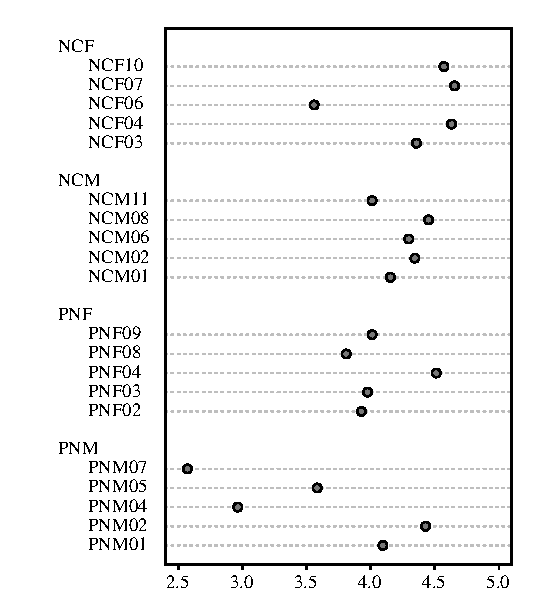
\includegraphics{figures/dotchart.eps}
	\caption[Intelligibility of talkers used to make the stimuli]{By-talker mean keywords correct (across dialect-matched listeners) in speech-shaped noise at +2 dB \ac{snr} (adapted from \citet{McCloyEtAl2013}).\label{fig:dotchart}}
	\end{centering}
\end{figure}

\begin{itm}
	\item{description of the sentences}
	\item{characterization of the talkers}
	\item{results of initial intelligibility study \& acoustic modeling}
	\item{method for selection of the 3 talkers used in the remainder of the experiments}
\end{itm}


\section{Stimulus design\label{sec:StimDesign}}
Why \ac{psola}?  Brief comparison of different methods for manipulating duration.  Malah1979 ("linearly combining adjacent intervals of speech to avoid major discontinuities in the waveform"), MoulinesCharpentier1990 (\ac{psola}).  Relate to the studies that used them: PichenyEtAl1989 (Malah method), UchanskiEtAl1996 (segment-by-segment time scaling), LiuZeng2006 (adding silences, "uniform scaling" = \ac{psola}?).  Cf KrauseBraida2002, KrauseBraida2004.

\begin{itm}
	\item{duration}
	\begin{itm}
		\item{forced alignment}
		\item{hand-correct forced alignment at syllable level}
		\item{auto extract syllable durations from textgrids}
	\end{itm}
	\item{pitch}
	\begin{itm}
		\item{semiauto pitch settings tool}
		\item{auto pitch object extraction}
		\item{auto manipulation from sound \& pitch (save as binary w/ sound)}
		\item{hand-correct pulses within manipulation}
		\item{auto extract point process from manipulation (as text)}
		\item{auto create pitch tier from point process (max interval 0.05s = 20Hz)}
		\item{auto replace pitch tier in manipulation object}
		\item{hand-correct pitch tier (spurious low pitch points)}
	\end{itm}
	\item{intensity}
	\begin{itm}
		\item{auto-extract intensity tier}
		\item{multiply target signal by its conjugate intensity contour}
		\item{dynamic time warp donor intensity contour to match target duration pattern}
		\item{multiply target signal by intensity contour of prosodic source}
	\end{itm}
	\item{PSOLA resynthesis}
	\begin{itm}
		\item{dynamic time warping of intensity tier, pitch tier, and target signal}
		\item{intensity replacement}
		\item{pitch replacement}
	\end{itm}
	\item{final stimulus creation}	
	\begin{itm}
		\item{\ac{rms} normalization}
		\item{create speech shaped noise}
		\item{mix signal and noise — justify chosen \ac{snr}}
		\item{discuss danger of doing \ac{snr} before \ac{rms} — target signal below threshold}
	\end{itm}
\end{itm}


\section{experiment sessions}
% Rationale for how much training to do:  
% \citep{YonanSommers2000}: Trained talkerID on 4 talkers (2M2F) over 2 days.  Each day: 60 exposure trials, 40 trials training w/ feedback, 60 more exp, 40 more training, 80 test.  All phases were half high-context and half low-context sentences.  End of day 2: single words \& sentences in SNR -5,0,+5, half high- half low-context, half familiar talkers half novel, half male talkers half female.  Familiar/unfamiliar talkers were piloted to make sure they were equally intelligible generally, and to old vs young people.  RESULTS: young listeners near ceiling on talkerID both day1 and day2; old listeners 73\% and 76\%.  Training on sentence material did not aid on the single word task (same as NygaardPisoni1998).  There was a benefit of familiar talker for sentence materials, which was stronger at lower SNRs.  A similar pattern obtained for a second experiment with talker exposure instead of talkerID training.
% \citep{VanEngen2012}: Two 30-minute training sessions (64 sentences) with noise (either SSN, English 2-babble, Mandarin 2-babble) and feedback.  Posttest 1 familiar, 1 unfamiliar talker, half in English babble, half in mandarin.  Trained and tested at their HINT threshold -3dB (based on VanEngen2010) to avoid floor/ceiling.  Results: “(1) listeners were able to take advantage of target talker familiarity; (2) training with babble was more effective than SSN training; and (3) after babble training, listeners improved most in coping with the babble in which they were trained [English or Mandarin]. In general, the results show that processes related both to tuning in to speech targets and tuning out speech maskers can be improved with auditory training”

Stimuli were presented with a stationary gaussian masker noise, frequency shaped to match the long term spectral average of the corpus of stimuli, at a +2 dB \ac{snr}.  To ensure target audibility, the level of the speech was held constant at 68 dB SPL (dB \ac{rms} in a 6 cc coupler) and the masker noise was digitally added to the speech to achieve the desired \ac{snr}.  The combined signal was presented in a sound-insulated booth over closed-back supra-aural headphones (Sennheiser HD 25–1 II).  Listeners were instructed to repeat each sentence they heard, to give partial answers when they only heard some words, and to guess when they were unsure.  Trials were scored 0–5 on keywords correct during the task.  An audio recording was made of listener responses, and scoring uncertainties were resolved offline by a second researcher.  Talker-sentence-\ac{snr} assignments were random and unique for each listener, with the following constraints: (a) each listener heard each talker an equal number of times; (b) within each talker, each listener heard each \ac{snr} an equal number of times; (c) each listener heard each sentence only once.

\begin{itm}
	\item{subjects}
	\begin{itm}
		\item{number of listeners}
		\item{hearing test}
		\item{dialect controls}
		\item{demographics: age, gender, ethnicity, geography}
		\item{English native; other languages?}
	\end{itm}
	\item{procedure}
	\begin{itm}
		\item{booth, headphones, presentation level}
		\item{task}
		\item{scoring}
	\end{itm}
\end{itm}

\section{data analysis}
\begin{itm}
	\item{mixed effects models (probably logistic)}
\end{itm}

\chapter{Results}

\section{Experiment 1}
Experiment~1 tests the role of prosody in intelligibility, by comparing mean sentence scores for unmodified talkers against resynthesized stimuli with prosodic replacement.  The mean sentence score for each talker across listeners is shown in Figure~\ref{fig:ExpOneBarplot}.  Darker bars indicate unmodified recordings, while light bars represent resynthesized stimuli.  Contrary to expectations, not all resynthesized stimuli have lower mean scores compared to their unmodified counterparts, suggesting that distortion due to the resynthesis process was relatively minimal.\footnotemark{}  With regard to Research Question~1 — how does prosody relate to intelligibility — a complicated picture emerges.  Talker~\ac{b} suffers dramatically when his prosody is replaced, whereas Talker~\ac{c} is unchanged or slightly improved, and Talker~\ac{a} is unchanged or slightly worsened.

\footnotetext{This is likely due to several factors.  One is probably the painstaking hand-correction of the pulse marking to ensure consistent phase throughout voiced spans of speech.  Another is the choice to maintain each talker’s natural mean pitch on each sentence, and map only the {\emph shape} of the pitch contour of the prosodic donor during resynthesis.}

One possible explanation for these results is to postulate that Talker~\ac{a}, despite being highly intelligible, does not have especially good prosody, evidenced in particular by the fact that scores for Talker~\ac{ca} are lower than the scores for Talker~\ac{cb}.  On the same grounds, and on the additional observation that scores for Talker~\ac{ab} are greater than for Talker~\ac{ac}, we might conclude that Talker~\ac{b} has more intelligible prosody than the other two talkers, and his middling base intelligibility scores are due to segmental factors.

\begin{figure}[htbp]
	\begin{centering}
	\includegraphics{figures/results/ExpOneBarplot.eps}
	\caption[Barplot of mean sentence scores for Experiment~1]{Barplot of mean sentence scores for Experiment~1.  Error bars are ±1 standard error; lighter colors indicate resynthesized talkers, with the second letter indicating the prosodic donor (see Section~\ref{sec:ExpDesign} for full explanation of talker codes).\label{fig:ExpOneBarplot}}
	\end{centering}
\end{figure}

With regard to the question of whether low-intelligibility talkers can be made more intelligible through prosody alone, it would appear that the answer is “yes”: Talker~\ac{cb} appears to have higher scores than Talker~\ac{c}, despite the likelihood that Talker~\ac{cb}’s recordings suffer some amount of distortion from the resynthesis process.  In other words, any detriment due to resynthesis is more than overcome by the benefit of having Talker~\ac{b}’s prosody.  

To further probe these results, the scores were submitted to a mixed-effects linear regression model, shown in Equation~\ref{eq:ExpOneMM}:

\begin{equation}\label{eq:ExpOneMM}
	\text{{\inlinecode lmer(sentScore\textasciitilde resynth+segDonor+proDonor+(1|listener)+(1|sentence), data=allData)}}
\end{equation}

In this model, {\inlinecode sentScore} is the number of keywords correct (0–5), {\inlinecode resynth} is a boolean variable that is true for Talkers~\ac{ab ac ba bc ca} and~\ac{cb}, and {\inlinecode segDonor} and {\inlinecode proDonor} are three-level factors indicating the talker in the target signal and the talker from whom the prosodic information was drawn, respectively.  For the unmodified original recordings, {\inlinecode segDonor} and {\inlinecode proDonor} are defined as the talker himself, even though those recordings were not resynthesized.  

A summary of the model shown in Equation~\ref{eq:ExpOneMM} is given in Table~\ref{tab:ExpOneFixedEff}.  There was no evidence of correlation of fixed effects (correlation coefficients ranged from 0 to 0.505; not shown in Table~\ref{tab:ExpOneFixedEff}).  The baseline condition is Talker~\ac{a}, with a value at the intercept of about 4.4 words correct.  The coefficients reveal similar patterns as Figure~\ref{fig:ExpOneBarplot}.  Firstly, the model supports the interpretation that Talker~\ac{b} has the most intelligible prosody: having the prosody of Talker~\ac{b} represents a net gain of 0.3 words correct over the prosody of Talker~\ac{a}, whereas having the prosody of Talker~\ac{c} represents a net loss of 0.6 words correct.  The model also supports the idea that Talker~\ac{a}’s intelligibility stems in large part from segmental factors, given that the other levels of {\inlinecode segDonor} both have strongly negative coefficients.

% TODO: fix rowfont bolding (currently not bolding) in this table and in Exp 2 table
\begin{table}
	\caption[Experiment~1 statistical model: Fixed effects]{Summary of fixed effect predictors in the statistical model of Experiment~1.\label{tab:ExpOneFixedEff}}
	\centering
	\begin{tabu} spread 1em {Xrcrc}
		\toprule
		\rowfont{\textbf}\multicolumn{5}{l}{Summary of fixed effects (N=1440; log-likelihood=-2554)}\\
		\rowfont[c]{\textbf}\multicolumn{1}{l}{Predictor} & Coefficient & \textit{SE} & \textit{t} & \textit{p}\\
		\midrule
		Intercept         &  4.382 & (0.132) &  33.19 & <10⁻¹⁶\\
		resynth = TRUE    & −0.666 & (0.077) &  −8.64 & <10⁻¹⁶\\
		segDonor = \ac{b} & −1.679 & (0.089) & −18.82 & <10⁻¹⁶\\
		segDonor = \ac{c} & −1.274 & (0.090) & −14.18 & <10⁻¹⁶\\
		proDonor = \ac{b} &  0.315 & (0.089) &   3.54 & <10⁻³\\
		proDonor = \ac{c} & −0.635 & (0.088) &  −7.19 & <10⁻¹¹\\
		\bottomrule
	\end{tabu}
\end{table}

A summary of the random effects in the model of Experiment~1 are shown in Table~\ref{tab:ExpOneRandomEff}.  The results are unremarkable: as expected, the variability of listeners is relatively low (s²=0.043, or a standard deviation of 0.2 keywords correct across listeners), suggesting that to a first approximation listeners are all equally good at the task.  In contrast, the variability of sentence difficulty is somewhat higher (s²=0.513, or a standard deviation of 0.7 keywords correct across sentences).

%Random effects:
% Groups   Name        Variance Std.Dev. MCMCmean   HPD95lower HPD95upper
% sent     (Intercept) 0.51345  0.71655  0.6040129  0.5055609  0.7081530
% listener (Intercept) 0.04289  0.20710  0.2212181  0.1082121  0.3494921
% Residual             1.78542  1.33620  1.3516454  1.3010096  1.4038710
\begin{table}
	\caption[Experiment~1 statistical model: Random effects]{Summary of random effects in the statistical model of Experiment~1.\label{tab:ExpOneRandomEff}}
	\centering
	\begin{tabu} spread 1em {Xcccc}
		\toprule
		\multicolumn{3}{l}{\bfseries Summary of random effects} & \multicolumn{2}{c}{95\% \ac{hpd}}\\
		Group & \textit{s}² & \ac{mcmc} mean & lower bound & upper bound\\
		\midrule
		Sentence (intercept) & (0.513) & 0.604 & 0.506 & 0.708\\
		Listener (intercept) & (0.043) & 0.221 & 0.108 & 0.349\\
		Residual             & (1.785) & 1.352 & 1.301 & 1.404\\
		\bottomrule
	\end{tabu}
\end{table}


\section{Experiment 2}
Experiment~2 tests the role of prosody in the familiar talker advantage, by comparing mean sentence scores for various talkers across two groups of listeners: those trained on one of the test talkers (Talker~\ac{c}), and those trained on a control talker (Talker~\ac{d}).  The first question to be addressed is whether the training phase was in fact effective for both groups of listeners.  Mean sentence scores of the training phase (grouped by quartile) are shown in Figure~\ref{fig:Quartile}. 

\begin{figure}[htbp]
	\begin{centering}
	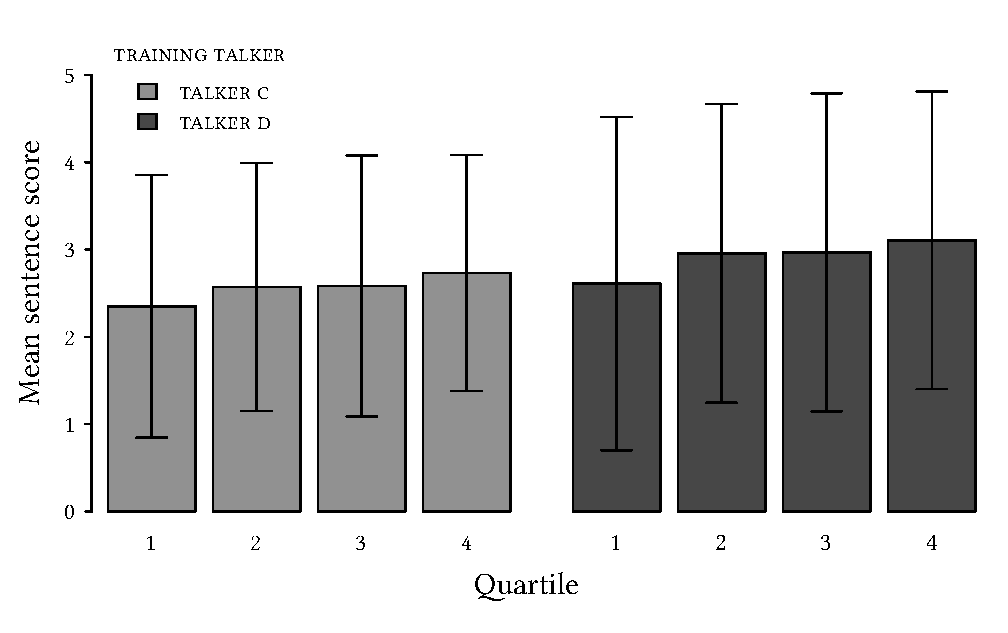
\includegraphics{figures/results/QuartileBarplot.eps}
	\caption[Quartile analysis of training phase in Experiment~2]{Quartile analysis of training phase in Experiment~2.  Improvement is seen during training for both the control group (trained on Talker~\ac{d}) and the test group (trained on Talker~\ac{c}).  The adaptation in the test group appears not to have been maintained during testing.\label{fig:Quartile}}
	\end{centering}
\end{figure}

T-tests performed on the first and fourth quartile of each group show a statistically significant improvement in both groups of listeners (control group: \textit{t}=−2.898 on 437.2 degrees of freedom, \textit{p}<0.01; test group: \textit{t}=−2.816 on 438.1 degrees of freedom, \textit{p}<0.01).  However, the improvement is small (less that 0.5 keywords for both groups), and more importantly it appears the adaptation that occurred during training was not fully retained during the testing phase, as evidenced by the slight decline in performance on Talker~\ac{c} during the testing phase when compared to the last quartile of the training phase (see Figure~\ref{fig:Quartile}).\footnotemark{}

footnotetext{This is true at least for the listeners trained on Talker~\ac{c}.  Listeners trained on Talker~\ac{d} did not hear their training talker during the testing phase, so it is unknown whether any adaptation was retained during testing.  Presumably, however, any such adaptation would have had little effect on performance when listening to Talkers~\ac{a}, \ac{b}, or \ac{c}.}

One explanation for the failure to retain a perceptual advantage between the training to the testing phases is stimulus uncertainty: in the training phase, listeners heard the same talker for 90 sentences in a row, whereas the testing phase comprised a random ordering of sentences from the three unmodified talkers and the six resynthesized talkers.  It is possible that the uncertainty due to varying the talkers negated any advantage acquired from the training.  Another possible explanation is that the training was too brief, and the apparent learning seen in the quartile analysis is merely a task familiarization effect that was not tied to any particular talker.

In light of the preceding discussion it is perhaps unsurprising that training on a particular talker did not confer a reliable perceptual advantage on test stimuli resynthesized to have the training talker’s prosody.  Full results of the statistical model for Experiment~2 are shown in Table~\ref{tab:ExpTwoFixedEff}.  Predictor codes are the same as in the model for Experiment~1, with the addition of {\inlinecode segTrain} (a boolean variable indicating match between the training talker and the segmental donor of the test stimulus) and {\inlinecode proTrain} (indicating match between the training talker and the prosodic donor of the test stimulus).

Aside from the two non-significant predictors {\inlinecode segTrain} and {\inlinecode proTrain}, the model is nearly identical to the model for Experiment~1; the magnitude, direction, and significance of the other predictors are all unchanged from Experiment~1.

\begin{table}
	\caption[Experiment~2 statistical model: Fixed effects]{Summary of fixed effect predictors in the statistical model of Experiment~2.\label{tab:ExpTwoFixedEff}}
	\centering
	\begin{tabu} spread 1em {Xrcrc}
		\toprule
		\rowfont{\textbf}\multicolumn{5}{l}{Summary of fixed effects (N=1800; log-likelihood=-3103)}\\
		\rowfont[c]{\textbf}\multicolumn{1}{l}{Predictor} & Coefficient & \textit{SE} & \textit{t} & \textit{p}\\
		\midrule
		Intercept	      &  4.334 & (0.129) &  33.56 & <10⁻¹⁶\\
		resynth = TRUE    & −0.604 & (0.066) &  −9.17 & <10⁻¹⁶\\
		segDonor = \ac{b} & −1.467 & (0.075) & −19.46 & <10⁻¹⁶\\
		segDonor = \ac{c} & −1.160 & (0.098) & −11.83 & <10⁻¹⁶\\
		proDonor = \ac{b} &  0.269 & (0.075) &   3.59 & <10⁻³\\
		proDonor = \ac{c} & −0.586 & (0.098) &  −5.98 & <10⁻⁸\\
		segTrain = TRUE   &  0.009 & (0.125) &   0.08 & 0.94\\
		proTrain = TRUE   & −0.115 & (0.125) &  −0.92 & 0.36\\
		\bottomrule
	\end{tabu}
\end{table}

A summary of the random effects in the model of Experiment~2 are shown in Table~\ref{tab:ExpTwoRandomEff}.  The results are again unremarkable: like the model for Experiment~1, the variability of listeners is relatively low (s²=0.083, or a standard deviation of 0.3 keywords correct across listeners), and the variability of sentence difficulty is again somewhat higher (s²=0.537, or a standard deviation of 0.7 keywords correct across sentences).

% Random effects:
% Groups   Name        Variance Std.Dev. MCMCmean   HPD95lower HPD95upper
% sent     (Intercept) 0.537497 0.73314  0.6170353  0.5238609  0.7132486
% listener (Intercept) 0.083091 0.28825  0.2972227  0.1879063  0.4192268
% Residual             1.616020 1.27123  1.2835182  1.2405740  1.3280362

\begin{table}
	\caption[Experiment~2 statistical model: Random effects]{Summary of random effects in the statistical model of Experiment~2.\label{tab:ExpTwoRandomEff}}
	\centering
	\begin{tabu} spread 1em {Xcccc}
		\toprule
		\multicolumn{3}{l}{\bfseries Summary of random effects} & \multicolumn{2}{c}{95\% \ac{hpd}}\\
		Group & \textit{s}² & \ac{mcmc} mean & lower bound & upper bound\\
		\midrule
		Sentence (intercept) & (0.537) & 0.617 & 0.524 & 0.713\\
		Listener (intercept) & (0.083) & 0.297 & 0.188 & 0.419\\
		Residual             & (1.616) & 1.284 & 1.241 & 1.328\\
		\bottomrule
	\end{tabu}
\end{table}

% TODO: check mismatch between binary and continuous models for experiment 2

% TODO: some closing remarks?

% TODO: post hoc: count release bursts?
% TODO: post hoc: pitch range, pitch dynamicity, intensity velocity, vowel space area?
% TODO: training with talker B



\chapter{Discussion}

\section{Future directions}
\begin{itm}
	\item{decomposing effects of prosodic dimensions}
	\begin{itm}
		\item{{\bfseries Experiment 5:} What are the relative contributions of duration, pitch, and intensity to talker intelligibility?  (Repeat of experiment 1 where only 1 or 2 of the dimensions are replaced via resynthesis.)}
	\end{itm}
	\item{talker ID studies}
	\begin{itm}
		\item{{\bfseries Experiment 6:} Can you train listeners to make a reliable talker ID distinction on the basis of prosody alone?  Can listeners reliably categorize B/C and B/A as different talkers?}
		\item{{\bfseries Experiment 7:} Can you train listeners to make a reliable talker ID distinction when prosody has been neutralized?  Can listeners reliably categorize C/B and A/B as different talkers?}
	\end{itm}
\end{itm}


\end{spacing}

% BIBLIOGRAPHY (SINGLE SPACED)
\bibliographystyle{apa-custom}
\bibliography{dissertation}

%\appendix
\titleformat{\chapter}{\LARGE\bfseries\doublespacing}{Appendix \thechapter.}{0.6em}{}
\begin{appendices}
\input{apx_HarvardSents}
\chapter{Praat scripts\label{apx:PraatScripts}}

% SEGMENTATION
\section{Syllabific segmentation by intensity}
This script takes a directory of sound files and, for each file, creates a new TextGrid and prepopulates an interval tier with boundaries at each local minimum of the sound file’s intensity contour.  It then presents the user with a TextGrid editor for the opportunity to adjust boundaries, add new ones, delete spurious ones, and add notes if desired.  The file name, notes (if any) and a sequential number are written to a log file.  Users can stop the script at any time, and resume work on the same directory of sound files by entering a “starting file number” when re-initiating the script.
\begin{code}
	\inputminted[fontsize=\footnotesize, tabsize=2]{r}{../scripts/CreateSyllableTierFromIntensity_DissVersion.praat}
	\caption[Syllabic segmentation by intensity]{Praat script for semi-automated syllable-level segmentation by intensity\label{lst:SylInt}}
\end{code}
\newpage

% PITCH SETTINGS AND PULSE CORRECTION
\section{Semi-auto pulse correction}
This script faciliates semi-automatic creation of manipulation objects from \texttt{.wav} files.  It takes a directory of sound files and, for each file, displays the pitch contour over a narrowband spectrogram, and prompts the user to either:
\begin{inparaenum}
	\item accept the pitch settings, 
	\item adjust the pitch floor/ceiling and redraw, or
	\item mark the file as unmeasurable,
\end{inparaenum}
before continuing on to the next file.  An \texttt{advancedInterface} option is available for users who want full control over all pitch parameters during the process.  Filename, duration, and pitch settings are saved to a tab-delimited log file.  The option \texttt{outputType} allows users to 
\begin{inparaenum}
	\item continue to next file after finalizing pitch settings,
	\item silently create and save manipulation objects using final pitch settings before continuing, or
	\item create manipulation objects and open them for hand-correction before continuing to the next file.
\end{inparaenum}  
\begin{code}
	\inputminted[fontsize=\footnotesize, tabsize=2]{r}{../scripts/SoundToManipulation_DissVersion.praat}
	\caption[Semi-auto pulse correction]{Praat script for semi-automated correction of glottal pulses within a manipulation object.\label{lst:PulseCor}}
\end{code}
\newpage

% PSOLA
\section{Prosody replacement with \psola}
This script takes as input two manipulation objects and two {TextGrids} and maps the pitch, duration, and intensity patterns from one manipulation object onto the other.  The manipulation objects must have the waveform embedded, but may be either text or binary.
\begin{code}
	\inputminted[fontsize=\footnotesize, tabsize=2]{r}{../scripts/ReplaceProsodyPSOLA_DissVersion.praat}
	\caption[Prosody replacement with \psola]{Praat script for prosodic replacement using \psola.\label{lst:ProsPSOLA}}
\end{code}

% CREATE LTAS NOISE
\section[Create speech-shaped noise]{Spectrally shape noise to match the long-term average spectrum of stimuli}
This script takes a directory of sound files, calculates the long-term average spectrum (\ac{ltas}) for each, and finds the average of the 
and, for each file, creates a new TextGrid and prepopulates an interval tier with boundaries at each local minimum of the sound file’s intensity contour.  It then presents the user with a TextGrid editor for the opportunity to adjust boundaries, add new ones, delete spurious ones, and add notes if desired.  The file name, notes (if any) and a sequential number are written to a log file.  Users can stop the script at any time, and resume work on the same directory of sound files by entering a “starting file number” when re-initiating the script.
\begin{code}
	\inputminted[fontsize=\footnotesize, tabsize=2]{r}{../scripts/CreateSyllableTierFromIntensity_DissVersion.praat}
	\caption[Syllabic segmentation by intensity]{Praat script for semi-automated syllable-level segmentation by intensity\label{lst:SylInt}}
\end{code}
\newpage

% ADD NOISE
\section{Mix signal and noise}
This script takes a directory of sound files and, for each file, creates a new TextGrid and prepopulates an interval tier with boundaries at each local minimum of the sound file’s intensity contour.  It then presents the user with a TextGrid editor for the opportunity to adjust boundaries, add new ones, delete spurious ones, and add notes if desired.  The file name, notes (if any) and a sequential number are written to a log file.  Users can stop the script at any time, and resume work on the same directory of sound files by entering a “starting file number” when re-initiating the script.
\begin{code}
	\inputminted[fontsize=\footnotesize, tabsize=2]{r}{../scripts/CreateSyllableTierFromIntensity_DissVersion.praat}
	\caption[Syllabic segmentation by intensity]{Praat script for semi-automated syllable-level segmentation by intensity\label{lst:SylInt}}
\end{code}
\newpage

% ADD NOISE
\section{Mix signal and noise}
This script takes a directory of sound files and, for each file, creates a new TextGrid and prepopulates an interval tier with boundaries at each local minimum of the sound file’s intensity contour.  It then presents the user with a TextGrid editor for the opportunity to adjust boundaries, add new ones, delete spurious ones, and add notes if desired.  The file name, notes (if any) and a sequential number are written to a log file.  Users can stop the script at any time, and resume work on the same directory of sound files by entering a “starting file number” when re-initiating the script.
\begin{code}
	\inputminted[fontsize=\footnotesize, tabsize=2]{r}{../scripts/CreateSyllableTierFromIntensity_DissVersion.praat}
	\caption[Syllabic segmentation by intensity]{Praat script for semi-automated syllable-level segmentation by intensity\label{lst:SylInt}}
\end{code}
\newpage


\end{appendices}
\end{document}
